% Figure -- beta-enrichment of the designable set (baseline vs REPA, 1.3M PDB).
% \input{} from Ch6 (sec:proteina-anatomy). Source: figures/scripts/fig_ch6_enrichment.py
\begin{figure}[tbp]
\centering
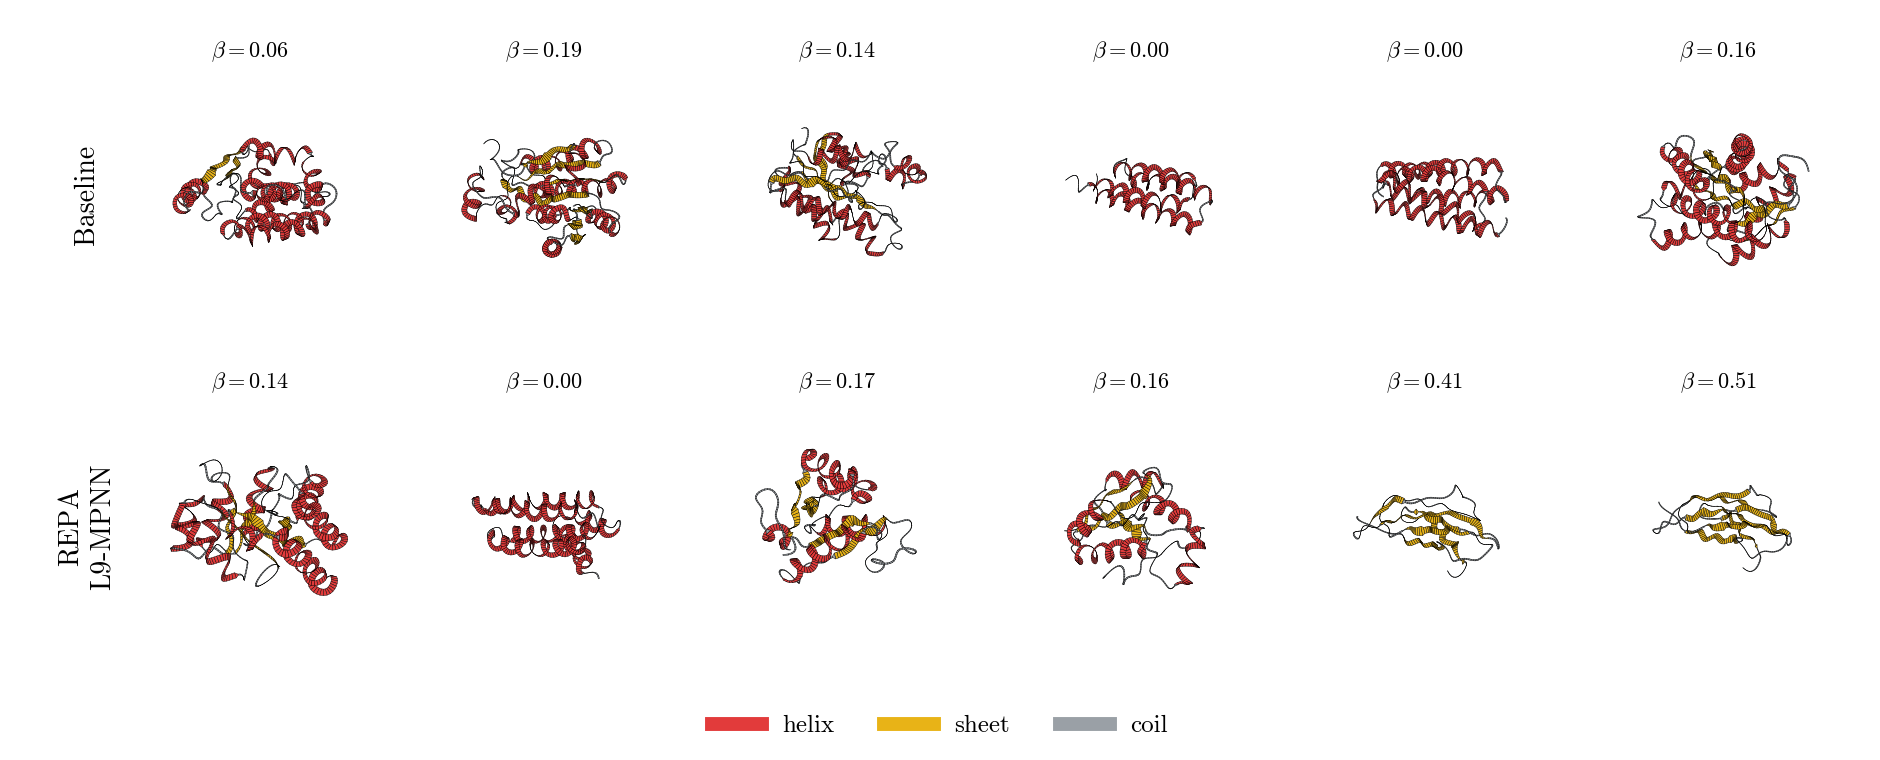
\includegraphics[width=\textwidth]{figures/fig_ch6_enrichment.png}
\caption{\textbf{On experimental data, REPA enriches the designable set for $\beta$-strand folds.} Designable backbones at 1.3M steps on experimental (PDB) data, coloured by secondary structure: baseline (top), REPA-L9-MPNN (bottom). Both produce helical folds, but REPA additionally yields $\beta$-rich folds (gold) the baseline rarely does, raising the designable $\beta$-strand fraction (Table~\ref{tab:proteina-13m}).}
\label{fig:proteina-enrichment}
\end{figure}
